% Class Notes Template
\documentclass[12pt]{article}
\usepackage[margin=1in]{geometry} 
\usepackage[utf8]{inputenc}

% Packages
\usepackage[french, english]{babel}
\usepackage{amsmath, amsthm, amssymb ,amsfonts, graphics, tikz, float, enumerate}
\usepackage{listings}
\usepackage{color} %red, green, blue, yellow, cyan, magenta, black, white
\definecolor{mygreen}{RGB}{28,172,0} % color values Red, Green, Blue
\definecolor{mylilas}{RGB}{170,55,241}

\lstset{language=Matlab,%
	%basicstyle=\color{red},
	breaklines=true,%
	morekeywords={matlab2tikz},
	keywordstyle=\color{blue},%
	morekeywords=[2]{1}, keywordstyle=[2]{\color{black}},
	identifierstyle=\color{black},%
	stringstyle=\color{mylilas},
	commentstyle=\color{mygreen},%
	showstringspaces=false,%without this there will be a symbol in the places where there is a space
	numbers=left,%
	numberstyle={\tiny \color{black}},% size of the numbers
	numbersep=9pt, % this defines how far the numbers are from the text
	emph=[1]{for,end,break},emphstyle=[1]\color{blue}, %some words to emphasise
	%emph=[2]{word1,word2}, emphstyle=[2]{style},    
}

% Title
\title{ECON 6130 - Problem Set \# 3}
\date{\today}
\author{Julien Manuel Neves}

% Use these for theorems, lemmas, proofs, etc.
\theoremstyle{definition}
\newtheorem{example}{Example}[section]
\newtheorem{theorem}{Theorem}
\newtheorem{lemma}[theorem]{Lemma}
\newtheorem{proposition}[theorem]{Proposition}
\newtheorem{claim}[theorem]{Claim}
\newtheorem{axiom}[theorem]{Axiom}
\newtheorem{corollary}[theorem]{Corollary}
\newtheorem{remark}[theorem]{Remark}
\newtheorem{definition}[theorem]{Definition}
\setcounter{MaxMatrixCols}{20}

% Usefuls Macros
\newcommand\N{\mathbb{N}}
\newcommand\E{\mathbb{E}}
\newcommand\R{\mathbb{R}}
\newcommand\F{\mathcal{F}}
\newcommand\Z{\mathbb{Z}}
\newcommand\st{\text{ such that }}
\newcommand\seq[1]{\{ #1 \}}
\newcommand{\inv}{^{-1}}


\newcommand{\norm}[1]{\|#1 \|}
\newcommand{\inp}[2]{\langle #1, #2 \rangle}

\newcommand{\pa}[1]{\left(#1\right)}
\newcommand{\bra}[1]{\left[#1\right]}
\newcommand{\cbra}[1]{\left\{#1\right\}}

\newcommand{\pfrac}[2]{\pa{\frac{#1}{#2}}}
\newcommand{\bfrac}[2]{\bra{\frac{#1}{#2}}}

\newcommand{\mat}[1]{\begin{matrix}#1\end{matrix}}
\newcommand{\pmat}[1]{\pa{\mat{#1}}}
\newcommand{\bmat}[1]{\bra{\mat{#1}}}


\begin{document}

\maketitle

\section*{Part (1)}


We use the following FRED series for our data:
\begin{enumerate}[(i)]
	\item Consumer Price Index of All Items in United States (USACPIALLQINMEI)
	\item Real Gross Domestic Product (GDPC1)
	\item Immediate Rates: Less than 24 Hours: Federal Funds Rate for the United States (IRSTFR01USQ156N)
	\item Unemployment Rate: Aged 15-64: All Persons for the United States (LRUN64TTUSQ156S)
\end{enumerate} 

The data are log-linearized the series and detrend with the Hodrick–Prescott filter. 

It is important to note that the Consumer Price Index represents the price level. Therefore, after taking the log of the CPI, it is important to differentiate the series before detrending them since
\[
\pi_t = \ln(P_t)-\ln(P_{t-1})
\]
where $P_t$ is the price level (CPI) at time $t$.

Moreover, for a measure of labor inputs, we need the following
\[
n_t = \ln\left( 1-\frac{U_t}{100}\right) 
\]
where $U_t$ is the unemployment rate in at time $t$ in per cent.

The detrended series are plotted in Fig.\ref{fig:data}.

\begin{figure}[H]
	\centering
	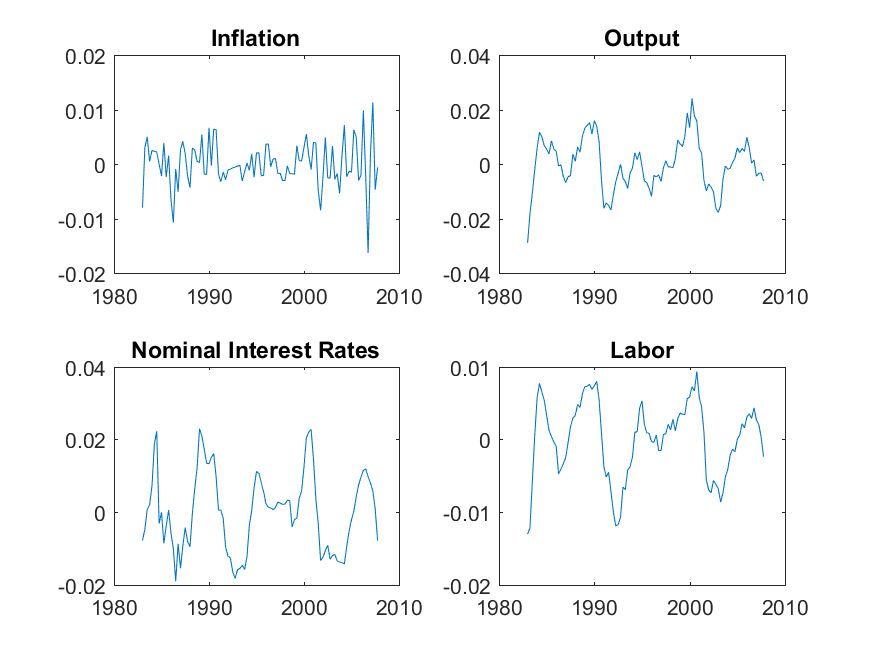
\includegraphics[width=\linewidth]{data}
	\caption{FRED Detrended Data}
	\label{fig:data}
\end{figure}

\section*{Part (2)}

Note that the equations for the New Keynesian business cycle can be listed as follows
\begin{align*}
\kappa\tilde{y}_t-\kappa x_t- u_t	& = 0\\
\pi_t-\beta \E_t(\pi_{t+1}) -\kappa {x}_t	-u_t& = 0\\
{x}_t - \E_t( {x}_{t+1}) + \frac{1}{\sigma}[(i_t-\rho)- \E_t(\pi_{t+1})-(r_t^e-\rho)]	& = 0\\
(r_t^e-\rho) +\sigma(1-\rho_a)\psi_{ya}a_t -(1-\rho_z)z_t	& = 0\\
(i_t-\rho) -\phi_{\pi}\pi_t -\phi_y\tilde{y}_t - \phi_y\psi_{ya} a_t-v_t	& = 0\\
v_t& = \rho_v v_{t-1} +\epsilon_t^v \\
a_t& = \rho_a a_{t-1}+\epsilon_t^a \\
z_t& = \rho_z z_{t-1}+\epsilon_t^z \\
u_t& = \rho_u u_{t-1}+\epsilon_t^u \\
{x}_{t}& =\E_{t-1}({x}_{t})+\eta_t^{{x}_t}\\
\pi_{t}& = \E_{t-1}(\pi_{t})+ \eta_t^{\tilde{n}} 
\end{align*}
where $\eta_t$ are the forecast errors.

Thus, we define the following states for our model
\[
S_t = [\tilde{y}_t, x_t,\pi_t,r_t^e-\rho,i_t-\rho,v_t,a_t,z_t,u_t,\E_t(x_{t+1}),\E_t(\pi_{t+1})]
\]

This implies the following parameters are need to be estimated/calibrated in order solve the model
\[
\Theta =\bmat{\sigma, \beta, \phi, \epsilon,\phi_\pi, \phi_y, \theta,\alpha, \rho_v,\rho_a,\rho_z,\rho_u,\sigma_v,\sigma_a,\sigma_z, \sigma_u}
\]
where the different parameters are defined as in Gali's book. In total, there is 16 parameters in our model.


\section*{Part (3)}

Note that our code is based on gensys.m which solves the following linear equation
\[
\Gamma_0 S_t = \Gamma_1 S_{t-1} + B +\Psi \epsilon_t + \Pi \eta_t
\]

Therefore, by rewriting the set of equations for the New Keynesian business cycle in matrix form, we get
\begin{align*}
\Gamma_0 &= \bmat{\kappa& -\kappa & 0 & 0& 0 &0 &0 &0 &-1 &0 &0\\
	0& -\kappa & 1 & 0& 0 &0 &0 &0 &-1 &0 &-\beta\\
	0& 1& 0& -\frac{1}{\sigma}&  \frac{1}{\sigma} & 0& 0  &0 &0 &-1& -\frac{1}{\sigma}\\
	-\phi_y &0 & -\phi_{\pi} & 0& 1& -1& -\phi_y\psi_{ya} &0& 0& 0&0\\
	0 &0 &0 &1 &0& 0& \sigma(1-\rho_a)\psi_{ya}& -(1-\rho_z) &0 &0 &0\\
	0& 0 &0 &0 &0 &1 &0& 0& 0 &0& 0\\
	0& 0 &0 &0 &0 &0 &1 &0 &0 &0& 0\\
	0& 0 &0 &0 &0 &0 &0 &1 &0 &0& 0\\
	0& 0 &0 &0 &0 &0 &0 &0 &1 &0& 0\\
	0 &1 &0 &0 &0 &0 &0 &0 &0& 0& 0\\
	0 &0 &1 &0 &0 &0 &0 &0& 0& 0& 0}\\
\Gamma_1 &= \bmat{0& 0 &0 &0& 0& 0& 0& 0& 0& 0& 0\\
	0& 0 &0& 0& 0& 0& 0 &0& 0 &0& 0\\
	0& 0 &0& 0& 0& 0 &0 &0 &0& 0& 0\\
	0& 0 &0& 0& 0& 0 &0 &0 &0 &0& 0\\
	0& 0 &0& 0& 0& \rho_v& 0 &0& 0& 0& 0\\
	0& 0 &0& 0& 0& 0 &\rho_a& 0& 0& 0 &0\\
	0& 0 &0& 0& 0& 0& 0 &\rho_z& 0& 0 &0\\
	0& 0 &0& 0& 0& 0& 0 & 0 &\rho_u& 0 &0\\
	0& 0 &0& 0& 0& 0& 0& 0& 0 &1 &0\\
	0& 0 &0& 0& 0& 0 &0 &0& 0& 0& 1}\\
\Psi    &= \bmat{0& 0 &0& 0 &0 &1 &0& 0& 0& 0& 0\\
	0& 0 &0& 0& 0& 0& 1 &0& 0& 0& 0\\
	0& 0 &0& 0& 0& 0& 0& 1& 0& 0& 0\\
	0& 0 &0& 0& 0& 0& 0& 0& 1& 0& 0}'\\
\Pi     &= \bmat{0& 0& 0& 0 &0 &0& 0& 0& 0& 1& 0\\
	0& 0& 0& 0& 0& 0& 0& 0& 0& 0& 1}'\\
B   &= \bmat{0& 0& 0& 0& 0& 0& 0& 0& 0& 0& 0}'
\end{align*}

Using theses matrices, gensys.m will ouput the coefficients of an $VAR(1)$ process of the following form
\[
S_t = A S_{t-1} + C \epsilon_t
\]
where $\epsilon_t\sim N(0,I)$.

Finally, to represents our model in state space form, we also need an equation that links the states to our observations. Since we have four exogenous shocks and four variables, we can write inflation, output, nominal interest rates, and labor in the following matrix form
\[
Z(t) = DX(t)
\]
where 
\[
D = \bmat{0& 0&1 &0& 0& 0& 0& 0& 0& 0& 0\\
	1& 0& 0& 0& 0& 0& \psi_{ya}& 0& 0& 0& 0\\
	0& 0& 0& 0& 1& 0& 0& 0& 0& 0& 0\\
	\frac{1}{1-\alpha}& 0& 0& 0& 0& 0& -\frac{1-\psi_{ya}}{1-\alpha}& 0& 0& 0& 0}
\]

See the appendix for the code.

\section*{Part (4)}

Note that the likelihood function for a state space model is given by
\[
L(\Theta \mid Z) = -\frac{pT}{2}\ln(2\pi) -\frac{1}{2}\sum_{t=1}^{T}\left[ \log(|\Omega_t|) + \tilde{Z}_t'\Omega_t\inv \tilde{Z}_t\right] 
\]
where $p$ is the number of observations and
\begin{align*}
	\tilde{Z}_t & = Z_t - DAX_{t-1\mid t-1}\\
	X_{t\mid t} & = AX_{t-1\mid t-1} + K_t\tilde{Z}_t\\
	\Omega_t & = DP_{t\mid t-1}D'+\Sigma_{vv}
\end{align*}

See the appendix for the code.
\section*{Part (5)}

The results for the maximum likelihood estimate of $\Theta$ are given in Tab.\ref{tab:sa}.
\begin{table}[H]
	\centering
\begin{tabular}{c|c}
	\hline
	& $\hat{\Theta}_{MLE}$\\
	\hline 
	$\sigma $   &  2.4596\\
	$\beta$     & 0.81704\\
	$\phi  $   &   3.0245\\
	$\epsilon$     &  5.2968\\
	$\phi_\pi $ &  1.5695\\
	$\phi_y $  & 0.64808\\
	$\theta $ &   0.65917\\
	$\alpha $  &  0.17379\\
	$\rho_v$   &  0.55141\\
	$\rho_a$  &   0.80006\\
	$\rho_z$  &   0.62\\
	$\rho_u$  &    0.38658\\
	$\sigma_v$&  0.0085544\\
	$\sigma_a$ &0.0038708\\
	$\sigma_z$ & 0.12524\\
	$\sigma_u$& 0.022965\\
	\hline 
\end{tabular}
	\caption{Simulated annealing estimation of New Keynesian model}
\label{tab:sa}
\end{table}


Note that for Tab.\ref{tab:sa}, we use the simulated code implemented in MATLAB. The results from the simulated annealing code used in class are reported in table Tab.\ref{tab:sa2}. 

While in both cases the impulses responses follow the same shape, the estimate are completely different. In fact, using the code shown in class, our estimates $\hat{\Theta}_{MLE}$ hits the upper bound that we set arbitrarily for $\beta $ and $\phi_\pi$. This is usually a bad sign and as such we discard these results. I would investigate this situation more deeply if I had more time.

\begin{table}[H]
	\centering
	\begin{tabular}{c|c}
		\hline
		& $\hat{\Theta}_{MLE}$\\
		\hline 
$\sigma $ &     0.35582\\
$\beta $   &  1\\
$\phi $     &       3.3888\\
$\epsilon$  &       6.5416\\
$\phi_\pi$  &         5\\
$\phi_y $  &   0.19053\\
$\theta$   &   0.72868\\
$\alpha $ & 0.23639\\
$\rho_v$   &  0.95112\\
$\rho_a$   &   0.83334\\
$\rho_z$   &    0.88805\\
$\rho_u$  &    0.60757\\
$\sigma_v$ &  0.026778\\
$\sigma_a$ & 0.0039169\\
$\sigma_z$ &  0.052927\\
$\sigma_u$ &   0.0071002\\
\hline 
	\end{tabular}
	\caption{Simulated annealing estimation of New Keynesian model (simannb.m)}
	\label{tab:sa2}
\end{table}


\section*{Part (6)}

The impulse responses are plotted in Fig.\ref{fig:impulse_monetary}, Fig.\ref{fig:impulse_prod}, Fig.\ref{fig:impulse_demand} and Fig.\ref{fig:impulse_cost}.

Note that the impulse response are plotted with respect to shocks of one unit in lieu of one standard deviation, i.e. we do not use $C$ for the impulse responses, but instead $C$ scaled down with the respective standard deviations of the shocks.

Moreover, for the estimation of output gap, we need the following measurement matrix in our state space model
\[
D = \bmat{0& 0&1 &0& 0& 0& 0& 0& 0& 0& 0\\
	1& 0& 0& 0& 0& 0& \psi_{ya}& 0& 0& 0& 0\\
	1& 0& 0& 0& 0& 0& 0& 0& 0& 0& 0\\
	0& 0& 0& 0& 1& 0& 0& 0& 0& 0& 0\\
	\frac{1}{1-\alpha}& 0& 0& 0& 0& 0& -\frac{1-\psi_{ya}}{1-\alpha}& 0& 0& 0& 0}
\]
\begin{figure}[H]
	\centering
	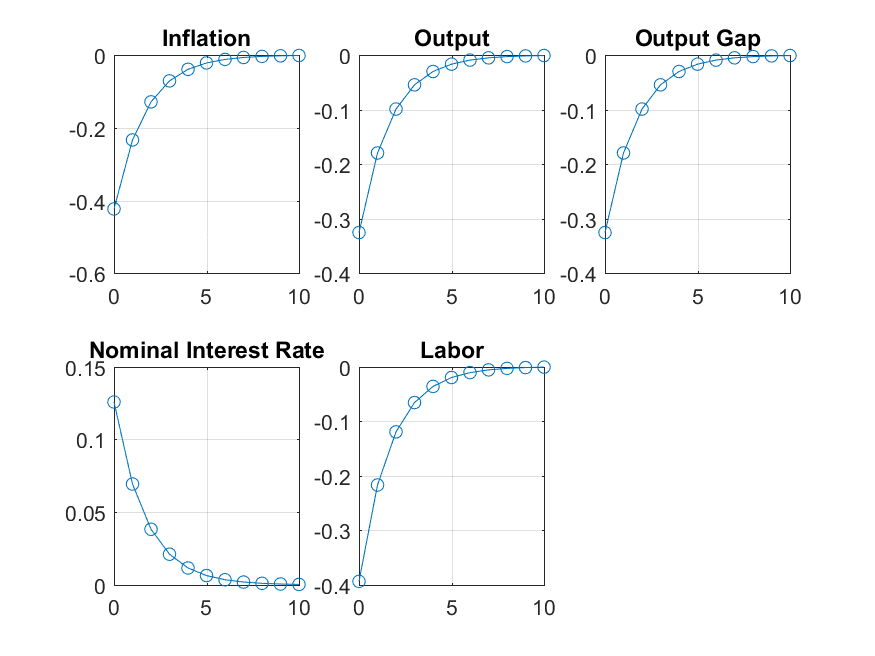
\includegraphics[width=\linewidth, height=0.4\textheight]{impulse_monetary}
	\caption{Impulse response to monetary shocks}
	\label{fig:impulse_monetary}
\end{figure}
\begin{figure}[H]
	\centering
	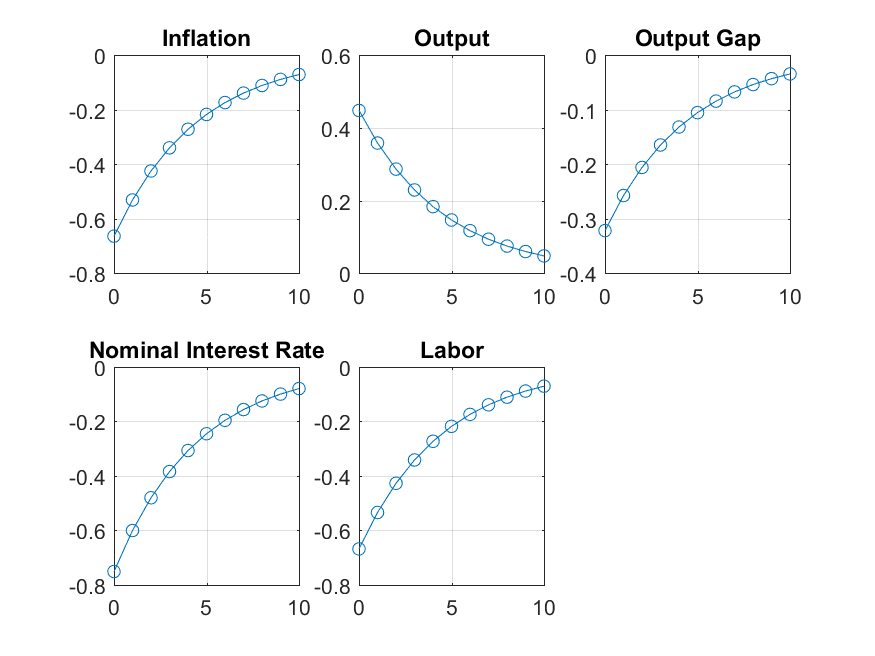
\includegraphics[width=\linewidth, height=0.4\textheight]{impulse_prod}
	\caption{Impulse response to productivity shocks}
	\label{fig:impulse_prod}
\end{figure}
\begin{figure}[H]
	\centering
	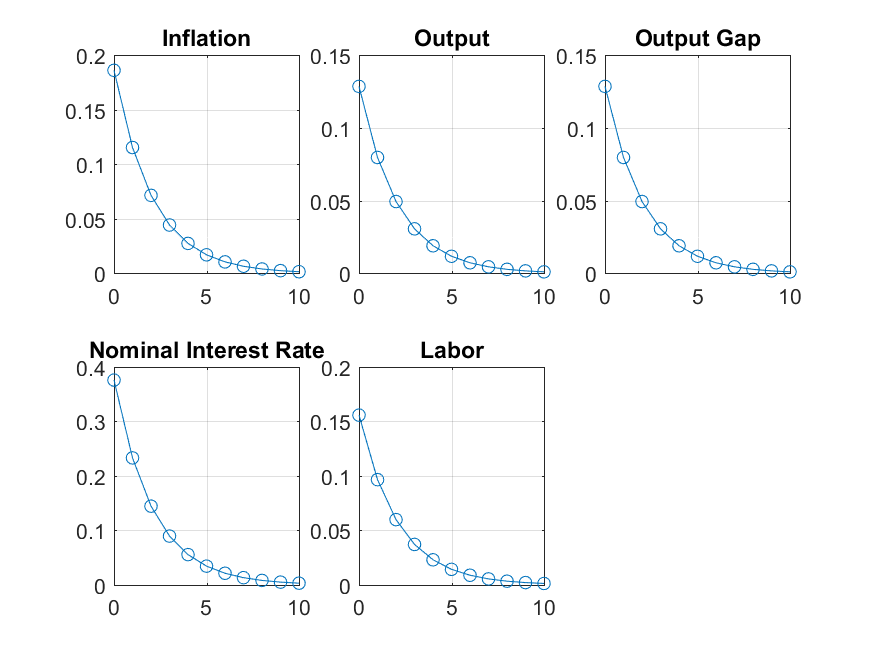
\includegraphics[width=\linewidth, height=0.4\textheight]{impulse_demand}
	\caption{Impulse response to demand shocks}
	\label{fig:impulse_demand}
\end{figure}
\begin{figure}[H]
	\centering
	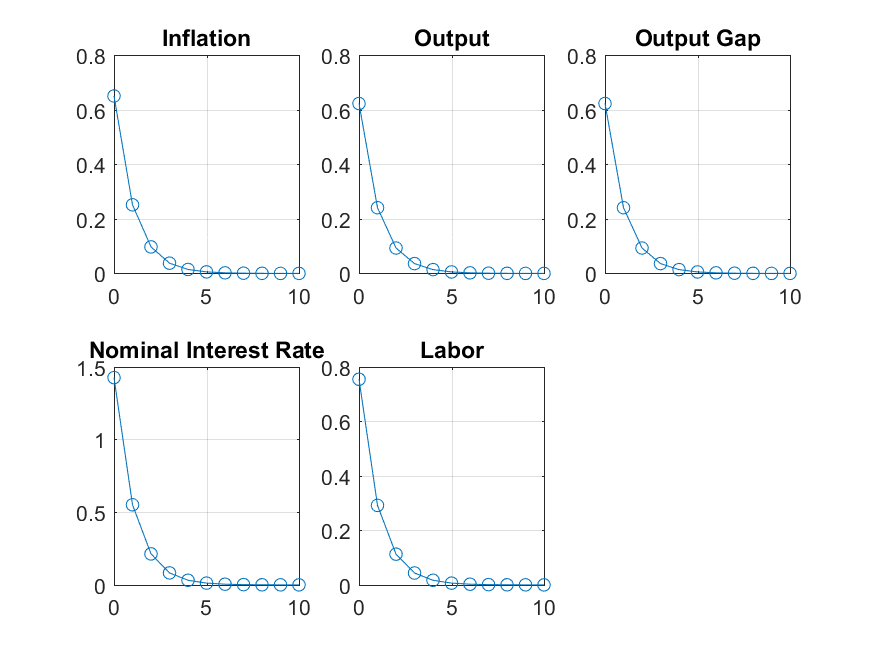
\includegraphics[width=\linewidth, height=0.4\textheight]{impulse_cost}
	\caption{Impulse response to cost-push shocks}
	\label{fig:impulse_cost}
\end{figure}

\section*{Part (7)}

Recall that we can write our model in the following state space form
\begin{align*}
S_t &= A S_{t-1} + C \epsilon_t\\
Z(t) &= DX(t)
\end{align*}
where $A$ and $C$ are defined as previously, $\epsilon_t\sim N(0,I)$, and
\[
D = \bmat{0& 0&1 &0& 0& 0& 0& 0& 0& 0& 0\\
	1& 0& 0& 0& 0& 0& \psi_{ya}& 0& 0& 0& 0\\
	0& 0& 0& 0& 1& 0& 0& 0& 0& 0& 0\\
	\frac{1}{1-\alpha}& 0& 0& 0& 0& 0& -\frac{1-\psi_{ya}}{1-\alpha}& 0& 0& 0& 0}
\]

Fig.\ref{fig:kalman} reports both the ouput and the estimated output gap.
\begin{figure}[H]
	\centering
	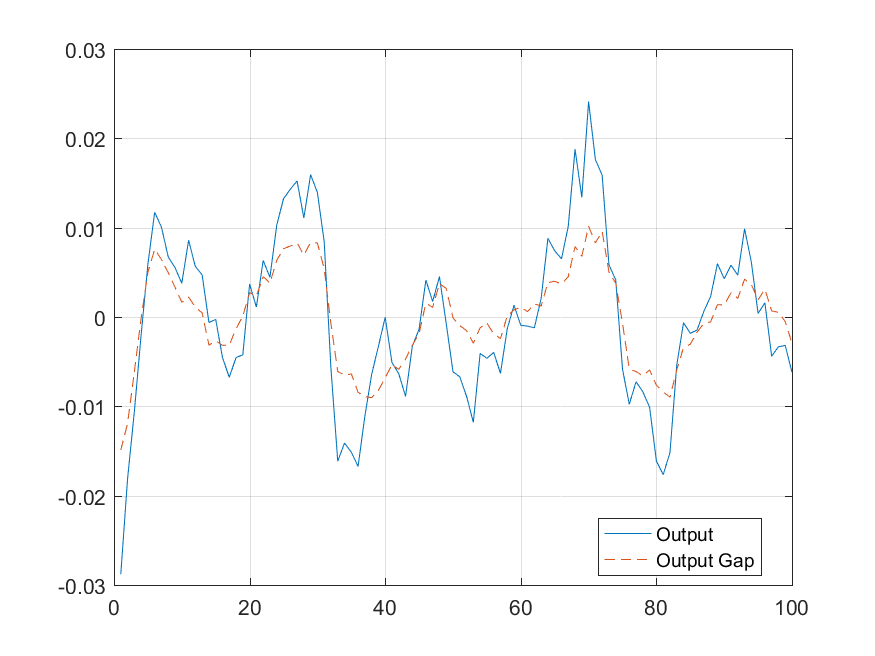
\includegraphics[width=\linewidth]{kalman}
	\caption{Kalman Filter estimate of output and output gap}
	\label{fig:kalman}
\end{figure}


\section*{Code}
\lstinputlisting[language=Matlab]{main.m}
\subsubsection*{New Keynesian Model (nkbc\_model.m)}
\lstinputlisting[language=Matlab]{nkbc_model.m}
\subsubsection*{Loglikelihood (loglikelihood\_DSGE.m)}
\lstinputlisting[language=Matlab]{loglikelihood_DSGE.m}
\subsubsection*{Kalman Filter (kfilter.m)}
\lstinputlisting[language=Matlab]{kfilter.m}

\end{document}
